\documentclass[a4paper,11pt]{article}
%\usepackage{polski}
\usepackage[cp1250]{inputenc}
\usepackage{latexsym}
\usepackage[ampersand]{easylist}
\usepackage{hyperref}
\usepackage{listings}
\usepackage{color}
\usepackage{graphicx}
\usepackage{sidecap}
\usepackage{wrapfig}
\usepackage[normalem]{ulem}

\author{W.~Kowalski}
\title{McSteel. User's manual}
\date{November 2020}
\frenchspacing


\begin{document}
\maketitle
%\begin{titlepage}
%{\huge McSafir}
%
%{\large User's manual}
%\end{titlepage}

\tableofcontents

\newpage
\section{Introduction}

Here will be general description of McSteel and its components.
Also short review of the software's feasibility.


\newpage
\section{Requirements}

McSteel is running only under Windows OS. Software was created and 
tested with Windows 10 Professional Edition. In the future Unix version
will be available.

McSteel is a set of Python scripts. Python 3.7 or higher are required.
The software has been tested with v3.7.0, v3.7.1 and v3.8.0. If you
notice any bugs in later versions, please inform authors of McSteel
raising a GitHub issue.
You can download Python from \url{https://www.python.org/downloads/}.

Essential software packages for McSteel to be run are listed below:
\begin{easylist}
\ListProperties(Start1=1)
& McOZone (multi\_zone) - full package \\\url{https://github.com/kowalskiw/multi_zone}
& SAFIR - demo version at least \\\url{https://www.uee.uliege.be/cms/c_4016386/en/safir}
& GiD - demo version at least \\\url{https://www.gidhome.com/}
& McSteel - full package \\\url{https://github.com/kowalskiw/mcsteel}
& text editor (i.e. Vim or Notepad++)
\end{easylist}
\newpage

\section{Running simulation}


\begin{wrapfigure}{l}{0.4\textwidth}
\begin{center}
\vspace{-20pt}
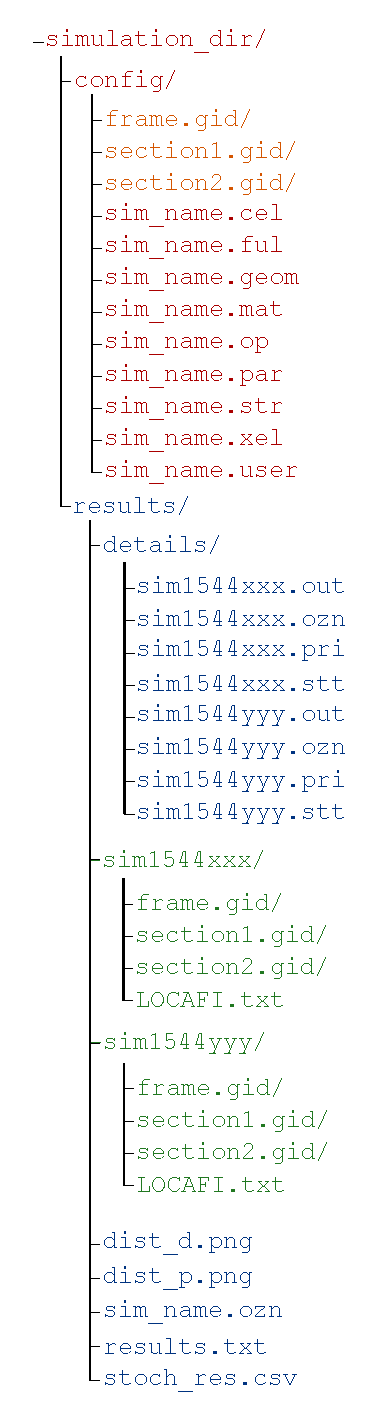
\includegraphics[scale=0.8]{dir_tree.pdf}
\end{center}
\vspace{-20pt}
\caption{Simulation directory structure.}
\vspace{-10pt}
\label{fig:dir_tree}
\end{wrapfigure}

McSteel is software package containing few partially-independent 
scripts. Some of them like i.e. McOZone's \emph{chart.py} or McSafir's 
\emph{fdsafir.py} scripts are able to work outside the package. You can 
also use McOZone or McSafir only. McSteel gather all this scripts
together and enable to reduce user involvement to projecting and 
setting up the configuration.

Therefore, this chapter treats of step by step instruction how to set
and conduct simulation using McSteel components.

\subsection{Directories tree}


Structure of directories and file's content is precisely defined.
Rules presented below should be respected in every step of analysis.
Figure \ref{fig:dir_tree} shows the tree of simulation directory.
Warm-colored elements need to be created by user (red - on his own, 
orange - using GiD). Blue-colored files and directories are created by
McOzone, and respectively green ones by McSAFIR. 

Main directory consists of two others: \emph{config} and \emph{results}.
The first one, with its whole content, is required to set up the 
simulation. Directories with \emph{.gid} extension should created using 
GiD (orange-colored). User specifies structure's geometry and 
properties (\emph{frame.gid}), sections' geometry and properties 
(\emph{section1.gid} and \emph{section2.gid}). This files will be
used to conduct FEM analyses \sout{and export as geometry as properties 
of construction to McOZone's files} (not implemented yet).
Red-colored files should be created on user's own in text editor. These 
are McOZone's configuration files and contains data needed to conduct 
multisimulation.





\clearpage
\newpage
\subsection{Creating model (GiD)}

\newpage
\subsection{Multisimulation (McOZone)}

\newpage
\subsection{Preparing ISO FEM analysis (SAFIR via GiD problemtypes)}

\newpage
\subsection{FEM analises (McSAFIR)}

\newpage
\section{Results and visualization}


\end{document}
